\documentclass[final,leqno,onetabnum]{siamltex0315}
\usepackage{amsfonts,amsmath,amssymb}
\usepackage{subfigure}
\usepackage{psfrag}
\usepackage{algorithmic}
\usepackage{algorithm}
\usepackage{lineno}

\makeatletter
\renewcommand{\ALG@name}{\sc Algorithm}
\makeatother

% Environments that will be called into the paper.

\newtheorem{assumption}[theorem]{\textit{Assumption}}
\newtheorem{remark}[theorem]{\textit{Remark}}

% Definitions used by included articles, reproduced here for 
% educational benefit, and to minimize alterations needed to be made
% in developing this sample file.

\newcommand{\pe}{\psi}
\def\d{\delta} 
\def\ds{\displaystyle} 
\def\e{{\epsilon}} 
\def\eb{\bar{\eta}}  
\def\enorm#1{\|#1\|_2} 
\def\Fp{F^\prime}  
\def\fishpack{{FISHPACK}} 
\def\fortran{{FORTRAN}} 
\def\gmres{{GMRES}} 
\def\gmresm{{\rm GMRES($m$)}} 
\def\Kc{{\cal K}} 
\def\norm#1{\|#1\|} 
\def\wb{{\bar w}} 
\def\zb{{\bar z}} 

% Some definitions used in the sample assumption.

\newcommand{\lW}[1]{\ensuremath{\lambda(W({#1},\rho))}}
\newcommand{\rhol}{\ensuremath{\rho_{\text{1,d}}}}
\newcommand{\rhoo}{\ensuremath{\rho_{\text{0,d}}}}
\newcommand{\ad}{\ensuremath{a_{\text{d}}}}
\newcommand{\rhoT}{\ensuremath{\rho_{\text{T,d}}}}

% Some definitions of bold math italics to make typing easier.
% They are used in the corollary.

\def\bfE{\mbox{\boldmath$E$}}
\def\bfG{\mbox{\boldmath$G$}}

% Line numbering to aid with review. Disabled before publication.

\linenumbers

% Title line. The thanks line in the title should be filled in if there
% is any support acknowledgement for the overall work to be included
% This \thanks is also used for the received by date info, but
% authors are not expected to provide this.

\title{eXample File for SIAM \LaTeX\ Macro Package\thanks{This 
        work was supported by the Society for Industrial and
        Applied Mathematics, Philadelphia, Pennsylvania.}}

\author{Sue Susans\thanks{Production Department, Society
        for Industrial and Applied Mathematics, 3600 Market St., 
        Philadelphia, PA 
        19104-2688 (\email{pseudonym@siam.org}, \email{alias@siam.org}).}
   \and James Jameson\footnotemark[2]
   \and A.~U.~Thors\thanks{Institute of Applied Mathematics, Department of
        Mathematics, Vancouver, BC V6T 1Z1, Canada (\email{au.thors@math.ubc.ca}).
        The research of this author was partially supported by various foundation grants.}}

\begin{document}

\maketitle

\begin{abstract}
An example of SIAM \LaTeX\ macros is presented. Various
aspects of composing manuscripts for SIAM's journal series
are illustrated with actual examples from accepted
manuscripts. SIAM's stylistic standards are adhered to
throughout and are illustrated.  When writing your own abstract, keep it to a single paragraph, avoid 
displayed math, and use standard TeX terms instead of your own definitions. 
\end{abstract}

\begin{keywords} 
sign-nonsingular matrix, LU-factorization, indicator
polynomial 
\end{keywords}

\begin{AMS}
15A15, 15A09, 15A23
\end{AMS}

\pagestyle{myheadings}
\thispagestyle{plain}
\markboth{S.~SUSANS, J.~JAMESON, AND A.~U.~THORS}{SIAM MACRO EXAMPLES}


\section{Introduction and examples}
This paper presents a sample file for the use of SIAM's
\LaTeX\ macro package. It illustrates the features of the
macro package, using actual examples culled from various
papers published in SIAM's journals. It is to be expected
that this sample will provide examples of how to use the
macros to generate standard elements of journal papers. This paper also
serves as an example of SIAM's stylistic preferences for
the formatting of such elements as bibliographic references,
displayed equations, and equation arrays, among others.  More information
about SIAM's editorial style can be found in the style manual, available
at \url{http://www.siam.org/journals/pdf/stylemanual.pdf}.

{\em Note:} This paper is not to be read in any form for content. 
The conglomeration of equations, lemmas, and other text elements were 
put together solely for typographic illustrative purposes and don't 
make any sense as lemmas, equations, etc.

\subsection{Sample text}
The following are a few sentences showing normal setup of math in text: Let $S=[s_{ij}]$ ($1\leq i,j\leq n$) be a $(0,1,-1)$-matrix
of order $n$. Then $S$ is a {\em sign-nonsingular matrix}
(SNS-matrix) provided that each real matrix with the same
sign pattern as $S$ is nonsingular. There has been
considerable recent interest in constructing and
characterizing SNS-matrices \cite{bs}, \cite{klm}, \cite{LiZeng2012a}. There
has also been interest in strong forms of
sign-nonsingularity \cite{djd}. In this paper we give a new
generalization of SNS-matrices and investigate some of
their basic properties.

Blackboard bold characters, such as $\mathbb{C}$ and $\mathbb{R}$, should be created with use of the {\tt amssymb} package and its definitions.
 
Let $S=[s_{ij}]$ be a $(0,1,-1)$-matrix of order $n$ and
let $C=[c_{ij}]$ be a real matrix of order $n$. The pair
$(S,C)$ is called a {\em matrix pair of order} $n$.
Throughout, $X=[x_{ij}]$ denotes a matrix of order $n$
whose entries are algebraically independent indeterminates
over the real field. Let $S\circ X$ denote the Hadamard
product (entrywise product) of $S$ and $X$. We say that the
pair $(S,C)$ is a {\em sign-nonsingular matrix pair of
order} $n$, abbreviated SNS-{\em matrix pair of order} $n$,
provided that the matrix \begin{linenomath*}\[A=S\circ X+C\]\end{linenomath*} is nonsingular
for all positive real values of the $x_{ij}$.  If $C=O$
then the pair $(S,O)$ is a SNS-matrix pair if and only if
$S$ is a SNS-matrix.  If $S=O$ then the pair $(O,C)$ is a
SNS-matrix pair if and only if $C$ is nonsingular. Thus
SNS-matrix pairs include both nonsingular matrices and
sign-nonsingular matrices as special cases.   Now  let $\alpha>0$ and let $x^*$ be the weak$^*$-limit of some net $\{x_\tau^*\}
  \subseteq (\sum_{i\in I}N_{C_i}(x))\cap\alpha\mathbf{B}$.
 
Matrices of no more than two rows appearing in text should be created with the commands {\tt atop}, 
{\tt choose}, or {\tt smallmatrix}: The multiplication is conformable at the block level, and the orthogonal
matrix $[ \begin{smallmatrix} B_{11} & B_{12} \\ B_{21} & B_{22} \end{smallmatrix} ]$,
said to be in \emph{bidiagonal-block form}, can be parameterized by
$\theta_{1},\dots,\theta_{r}\in[0,\frac{\pi}{2}]$ and $\phi_{1},\dots,\phi_{r-1}\in[0,\frac{\pi}{2}]$.  Matrices with three or more
rows should be used in display equations: The pairs $(S,C)$ with
\begin{linenomath*}
\[S=\left[\begin{array}{cc}1&0\\0&0\end{array}\right],\qquad 
C=\left[\begin{array}{cc}1&1\\1&1\end{array}\right]\] and 
\[S=\left[\begin{array}{ccc}1&1&0\\1&1&0\\0&0&0\end{array}\right],\qquad 
C=\left[\begin{array}{ccc}0&0&1\\0&2&0\\
3&0&0\end{array}\right]\]
\end{linenomath*}
are examples of SNS-matrix pairs.  

\subsection{A remuneration list}
In this paper we consider the evaluation of integrals of the 
following forms:
\begin{linenomath*}
\begin{equation}
\int_a^b \left( \sum_i E_i B_{i,k,x}(t) \right)
         \left( \sum_j F_j B_{j,l,y}(t) \right) dt,\label{problem}
\end{equation}
\end{linenomath*}
\begin{linenomath*}
\begin{equation}
\int_a^b f(t) \left( \sum_i E_i B_{i,k,x}(t) \right) dt,\label{problem2}
\end{equation}
\end{linenomath*}
where $B_{i,k,x}$ is the $i$th B-spline of order $k$ defined over the
knots $x_i, x_{i+1}, \ldots, x_{i+k}$.
We will consider B-splines normalized so that their integral is one.
The splines may be of different orders and
defined on different knot sequences $x$ and $y$.
Often the limits of integration will be the entire real line, $-\infty$
to $+\infty$. Note that (\ref{problem}) is a special case of (\ref{problem2})
where $f(t)$ is a spline \cite{BDM}.


There are five different methods for calculating (\ref{problem})
that will be considered:
\begin{remunerate}
\item Use Gauss quadrature on each interval.
\item Convert the integral to a linear combination of
      integrals of products of B-splines and provide a recurrence for
      integrating the product of a pair of B-splines.
\item Convert the sums of B-splines to piecewise
      B\'{e}zier format and integrate segment
      by segment using the properties of the Bernstein polynomials.
\item Express the product of a pair of B-splines as a linear combination
      of B-splines.
      Use this to reformulate the integrand as a linear combination
      of B-splines, and integrate term by term.
\item Integrate by parts.
\end{remunerate}
Of these five, only methods 1 and 5 are suitable for calculating 
(\ref{problem2}). The first four methods will be touched on and the 
last will be discussed at length.


\subsection{Some displayed equations and {\tt \{eqnarray\}}s}
     By introducing the product topology on  $R^{m \times m} \times
R^{n \times n}$  with the induced inner product
\begin{linenomath*}
\begin{equation}
\langle (A_{1},B_{1}), (A_{2},B_{2})\rangle := \langle A_{1},A_{2}\rangle 
+ \langle B_{1},B_{2}\rangle,\label{eq2.10}
\end{equation}
\end{linenomath*}
we calculate the Fr\'{e}chet derivative of  $F$  as follows:
\begin{linenomath*}
\begin{eqnarray}
 F'(U,V)(H,K) &=& \langle R(U,V),H\Sigma V^{T} + U\Sigma K^{T} -
P(H\Sigma V^{T} + U\Sigma K^{T})\rangle \nonumber \\
         &=& \langle R(U,V),H\Sigma V^{T} + U\Sigma K^{T}\rangle \label{eq2.11} \\
&=& \langle R(U,V)V\Sigma^{T},H\rangle + \langle \Sigma^{T}U^{T}R(U,V),K^{T}\rangle.     \nonumber
\end{eqnarray}
\end{linenomath*}
In the middle line of (\ref{eq2.11}) we have used the fact that the range of
$R$ is always perpendicular to the range of $P$.  The gradient $\nabla F$  of
$F$, therefore,  may be interpreted as the
pair of matrices:
\begin{linenomath*}
\begin{equation}
 \nabla F(U,V) = (R(U,V)V\Sigma^{T},R(U,V)^{T}U\Sigma ) \in
R^{m \times m} \times R^{n \times n}.       			\label{eq2.12}
\end{equation}
\end{linenomath*}
Because of the product topology, we know
\begin{linenomath*}
\begin{equation}
 {\cal T}_{(U,V)}({\cal O} (m) \times {\cal O} (n)) =
{\cal T}_{U}{\cal O} (m) \times {\cal T}_{V}{\cal O} (n),  		\label{eq2.13}
\end{equation}
\end{linenomath*}
where  ${\cal T}_{(U,V)}({\cal O} (m) \times {\cal O} (n))$  stands for the
tangent space to the manifold  ${\cal O} (m) \times {\cal O} (n)$  at  $(U,V)
\in {\cal O} (m) \times {\cal O} (n)$  and so on.  The projection of
$\nabla F(U,V)$  onto  ${\cal T}_{(U,V)}({\cal O} (m) \times {\cal O} (n))$,
therefore, is the product of the projection of the first component of
$\nabla F(U,V)$  onto  ${\cal T}_{U}{\cal O} (m)$  and the projection of the
second component of  $\nabla F(U,V)$  onto  ${\cal T}_{V}{\cal O} (n)$. 
In particular, we claim that the
projection $ g(U,V)$  of the gradient  $\nabla F(U,V)$  onto
${\cal T}_{(U,V)}({\cal O} (m) \times {\cal O} (n))$  is given by the pair of
matrices:
\begin{linenomath*}
\begin{eqnarray}
g(U,V) = && \left( \frac{R(U,V)V\Sigma^{T}U^{T}-U\Sigma V^{T}R(U,V)^{T}}{2}U,
\right.			\nonumber \\[-1.5ex]
\label{eq2.14}\\[-1.5ex]
&&\quad \left. \frac{R(U,V)^{T}U\Sigma V^{T}-V
   \Sigma^{T}U^{T}R(U,V)}{2}V \right).\nonumber
\end{eqnarray}
\end{linenomath*}
Thus, the vector field
\begin{linenomath*}
\begin{equation}
\frac{d(U,V)}{dt} = -g(U,V) 	\label{eq2.15}
\end{equation}
\end{linenomath*}
defines a steepest descent flow on the manifold  ${\cal O} (m) \times
{\cal O} (n)$ for the objective function  $F(U,V)$.

 
\section{Environments}\label{S2}
 
Let $(S,C)$ be a matrix pair of order $n$.  The determinant
\[\det (S\circ X+C)\] 
is a polynomial in the indeterminates of $X$ of degree at
most $n$ over the real field. We call this polynomial the
{\em indicator polynomial} of the matrix pair $(S,C)$
because of the following proposition.
 
\begin{theorem}[see \cite{SS13}]
\label{th:prop} 
The matrix pair $(S,C)$ is a {\rm SNS}-matrix pair if and
only if all the nonzero coefficients in its indicator
polynomial have the same sign and there is at least one
nonzero coefficient.
\end{theorem} 
 
\begin{proof}
Assume that $(S,C)$ is a SNS-matrix pair.  Clearly the
indicator polynomial has a nonzero coefficient.  Consider a
monomial
\begin{linenomath*}
\begin{equation} 
\label{eq:mono} 
b_{i_{1},\ldots,i_{k};j_{1},\ldots,j_{k}}x_{i_{1}j_{1}}\cdots
x_{i_{k}j_{k}}
\end{equation} 
\end{linenomath*}
occurring in the indicator polynomial with a nonzero
coefficient.  By taking the $x_{ij}$ that occur in
(\ref{eq:mono}) large and all others small, we see that any
monomial that occurs in the indicator polynomial with a
nonzero coefficient can be made to dominate all others.
Hence all the nonzero coefficients have the same sign. The
converse is im-\linebreak mediate. \qquad\end{proof} 
 

For SNS-matrix pairs $(S,C)$ with $C=O$ the indicator
polynomial is a homogeneous polynomial of degree $n$. In
this case Theorem \ref{th:prop} is a standard fact about
SNS-matrices.
 
\begin{lemma}[{\rm stability}]
\label{stability}
Given $T>0$, suppose that $\| \epsilon (t) \|_{1,2} \leq h^{q-2}$
for $0 \leq t \leq T$ and $q \geq 6$. 
Then there exists a positive number $B$ that depends on
$T$ and the exact solution $\pe$ only such that for all $0 \leq t \leq T$,
\begin{linenomath*}
\begin{equation}
\label{Gron}
\frac {d}{dt} \| \epsilon (t) \| _{1,2}  \leq B
   ( h^{q-3/2} + \| \epsilon (t) \|_{1,2})\;.
\end{equation}
\end{linenomath*}
The function $B(T)$ can be chosen to be nondecreasing in time.
\end{lemma}
 
 
\begin{theorem} 
\label{th:gibson} 
The maximum number of nonzero entries in a {\rm SNS}-matrix
$S$ of order $n$ equals \[\frac{n^{2}+3n-2}{2}\] with
equality if and only if there exist permutation matrices
such that $P|S|Q=T_{n}$ where
\begin{linenomath*}
\begin{equation} 
\label{eq:gibson} 
T_{n}=\left[\begin{array}{cccccc} 1&1&\cdots&1&1&1\\
1&1&\cdots&1&1&1\\ 0&1&\cdots&1&1&1\\ 
\vdots&\vdots&\ddots&\vdots&\vdots&\vdots\\ 
0&0&\cdots&1&1&1\\ 0&0&\cdots&0&1&1\end{array}\right]. 
\end{equation} 
\end{linenomath*}
\end{theorem} 
 
We note for later use that each submatrix of $T_{n}$ of
order $n-1$ has all 1s on its main diagonal. 
 
We now obtain a bound on the number of nonzero entries of
$S$ in a SNS-matrix pair $(S,C)$ in terms of the degree of
the indicator polynomial. We denote the strictly upper
triangular (0,1)-matrix of order $m$ with all 1s above the
main diagonal by $U_{m}$. The all 1s matrix of size $m$ by
$p$ is denoted by $J_{m,p}$.
 
 
\begin{proposition}[{\rm convolution theorem}]
\label{pro:2.1}  Let
\begin{linenomath*}
\begin{eqnarray*}
a\ast u(t) = \int_0^t a(t- \tau) u(\tau) d\tau, \hspace{.2in} t \in
(0, \infty).
\end{eqnarray*}
Then
\begin{eqnarray*}
\widehat{a\ast u}(s) = \widehat{a}(s)\widehat{u}(s).
\end{eqnarray*}
\end{linenomath*}
\end{proposition}

\begin{lemma}
\label{lem:3.1}
For $s_0 >0$, if
\begin{linenomath*}
$$
\int_0^{\infty} e^{-2s_0 t}v^{(1)}(t) v(t) dt \; \leq 0 \;,
$$
\end{linenomath*}
then
\begin{linenomath*}
\begin{eqnarray*}
\int_0^{\infty} e^{-2s_0 t} v^2(t) dt \; \leq \; \frac{1}{2s_0} v^2(0).
\end{eqnarray*}
\end{linenomath*}
\end{lemma}

\begin{corollary}\label{c4.1}
Let $ \bfE $ satisfy $(5)$--$(6)$ and
suppose $ \bfE^h $ satisfies $(7)$ and $(8)$
with a general $ \bfG $.  Let $ \bfG= \nabla \times {\bf \Phi} + \nabla p,$
$p \in H_0^1 (\Omega) $. Suppose that $\nabla p$ and $ \nabla \times 
{\bf \Phi} $ satisfy all the assumptions of Theorems {\rm \ref{th:prop}} and  
{\rm \ref{th:gibson}}, respectively. In addition suppose all the regularity
assumptions of Theorems {\rm \ref{th:prop}} and  
{\rm \ref{th:gibson}} are satisfied.  Then 
for $ 0 \le t \le T $ and $ 0 < \epsilon \le \epsilon_0 $ there exists a 
constant $ C = C(\epsilon, T) $ such that
\begin{linenomath*}
$$
\Vert (\bfE - \bfE^h)(t) \Vert_0 \le C h^{k+1- \epsilon},
$$
\end{linenomath*}
where $ C $ also depends on the constants given in Theorems 
$4.1$ and $4.2$.
\end{corollary}


\begin{definition}
{\rm Let $S$ be an isolated invariant set with isolating neighborhood $N$.
An {\em index pair} for $S$ is a pair of compact sets $(N_{1},N_{0})$
with $N_{0} \subset N_{1} \subset N$ such that:
\begin{romannum}
\item $cl(N_{1} \backslash N_{0})$
is an isolating neighborhood for $S$.
\item $N_{i}$ is positively invariant relative to $N$ for $i=0,1$,
i.e., given
$x \in N_{i}$ and $x \cdot [0,t] \subset N$, then $x \cdot [0,t] \subset
N_{i}$.
\item $N_{0}$ is an exit set for $N_{1}$, i.e. if $x \in N_{1}$,
$x \cdot [0, \infty ) \not\subset N_{1}$, then there is a $T \geq 0$ such
that $x \cdot [0,T] \subset N_{1}$ and $x \cdot T \in N_{0}$.
\end{romannum}}
\end{definition}

SIAM's preferred style for environments such as remarks, assumptions, and examples is italic lowercase headings and roman text.  They can be formatted by adding the line 
\begin{verbatim}{\newtheorem{remark}[theorem]{\textit{Remark}}\end{verbatim} (as appropriate) to the preamble.  The body of each remark is made italic with the command \texttt{rm}.

\begin{remark}[Lagrange multipliers]{\rm
The multipliers $p,\,p_{1},\,p_{2}$ are the Lagrange multipliers for the given constraints. The Lagrange multiplier $p$ represents the PDE constraint, the multiplier $p_{1}$ gives the dependency
 of the initial control $w$ to the initial condition $\rho(0,\cdot),$ and, finally, $p_{2}$ represents the relation between the control $a$ and the inflow $\lW{\cdot}\rho(\cdot,0)$.}\end{remark}

\begin{assumption}[compatibility conditions on  $\ad,\rhoo$ and $\rhol,\rhoT$ and the weights in the cost functional]\label{ass:compatibility}{\rm
For continuity reasons, we require the two compatibility conditions
\begin{linenomath*}
\[
 \ad(0)=\lambda(W(0,\rhoo))\,\rhoo(0),\qquad \rhol(T)=\rhoT(1)
\]
\end{linenomath*}
to hold at the origin $(0,0)$ and at the final point $(T,1)$, respectively, and the conditions on the weights in the cost functional, that is,
\begin{linenomath*}
\[
 \alpha=\lambda(W(0,\rhoo))^{-1}\,\epsilon,\qquad\gamma=\delta.
\]
\end{linenomath*}
}\end{assumption}

There is no default style for algorithms in the macro at present, but the preferred style would have a heading like that for theorems, i.e., small caps.  The body of the algorithm, if not
code, may be either italic or roman.  The following sample uses the \texttt{algorithm} style package, with the addition of a definition to change the appearance of the heading.
\begin{algorithm}
\caption{\hspace*{-4.3pt}{.} $T = \operatorname{BuildTree}(d,p)$.}
\label{alg:buildtree}
\begin{algorithmic}
\STATE{Define $P:=T:=\{ \{1\},\ldots,\{d\}$\}}
\WHILE{$\#P > 1$}
\STATE{Choose $C^\prime\in\mathcal{C}_p(P)$ with $C^\prime := \operatorname{argmin}_{C\in\mathcal{C}_p(P)} \varrho(C)$}
\STATE{Find an optimal partition tree $T_{C^\prime}$ }
\STATE{Update $P := (P{\setminus} C^\prime) \cup \{ \bigcup_{t\in C^\prime} t \}$}
% \STATE{Update $T := T \cup \{ \bigcup_{t\in\tau} t: \tau\in T_{C^\prime}{\setminus}\mathcal{L}(T_{C^\prime}) \}$}
\STATE{Update $T := T \cup \{ \bigcup_{t\in\tau} t : \tau\in T_{C^\prime}{\setminus} \mathcal{L}(T_{C^\prime})\}$}
\ENDWHILE
\RETURN $T$
\end{algorithmic}
\end{algorithm}

\subsection{Numerical experiments, with figures and tables} We conducted numerical experiments 
in computing inexact Newton steps for discretizations of a  
{\em modified Bratu problem}, given by  
\begin{linenomath*}
\begin{eqnarray} 
{\ds \Delta w + c e^w + d{ {\partial w}\over{\partial x} } } 
&=&{\ds f \quad {\rm in}\ D, }\nonumber\\[-1.5ex]
\label{bratu} \\[-1.5ex]
{\ds w }&=&{\ds 0 \quad {\rm on}\ \partial D , } \nonumber
\end{eqnarray}
\end{linenomath*} 
where $c$ and $d$ are constants. The actual Bratu problem has $d=0$ and  
$f \equiv0$. It provides a simplified model of nonlinear diffusion  
phenomena, e.g., in combustion and semiconductors, and has been 
considered by Glowinski, Keller, and Rheinhardt \cite{GloKR85}, 
as well as by a number of other investigators; see \cite{GloKR85} 
and the references therein. See also problem 3 by Glowinski and  Keller  
and problem 7 by Mittelmann in the collection of nonlinear model 
problems assembled by Mor\'e \cite{More}. The modified problem  
(\ref{bratu}) has been used as a test problem for inexact Newton 
methods by Brown and Saad \cite{Brown-Saad1}.  
 
In our experiments, we took $D = [0,1]\times[0,1]$, $f \equiv0$, 
$c=d=10$, and discretized (\ref{bratu}) using the usual second-order 
centered differences over a $100\times100$ mesh of equally 
spaced points in $D$. In \gmres($m$), we took $m=10$ and used fast  
Poisson right preconditioning as in the experiments in section \ref{S2}. The computing  
environment was as described in section \ref{S2}. All computing was done  
in double precision.  
 
 

In the first set of experiments, we allowed each method to  
run for $40$ {\gmresm} iterations, starting with zero as the initial  
approximate solution, after which the limit of residual norm  
reduction had been reached. The results are shown in Figure~\ref{f1}.  
In Figure~\ref{f1}, the top curve was produced by method FD1. 
The second curve from the top is actually a superposition of  
the curves produced by methods EHA2 and FD2; the two curves are 
visually indistinguishable. Similarly, the third curve from  
the top is a superposition of the curves produced by methods EHA4 
and FD4, and the fourth curve from the top, which lies barely above  
the bottom curve, is a superposition of the curves produced by  
methods EHA6 and FD6. The bottom curve was produced by method A. 


\begin{figure}
\centering \subfigure[$\epsilon_{\textnormal{max}} =
5\%$]{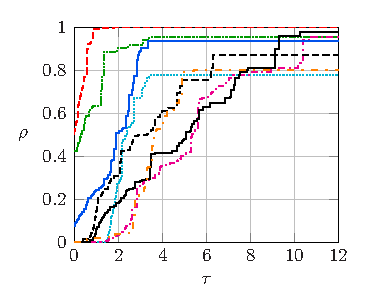
\includegraphics{lexample_fig1}}\qquad
\subfigure[$\epsilon_{\textnormal{max}} =
0.5\%$]{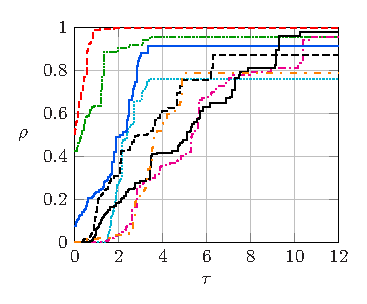
\includegraphics{lexample_fig2}} \caption[]{Avoid use of low line weights and light colors, which 
tend to disappear during printing.  Compare with Figure {\rm \ref{f2}}.}
\label{f1}
\end{figure}

\begin{figure}
\psfrag{lambda1}{\scriptsize$\lambda^2=1$}
\psfrag{lambda2}{\scriptsize$\lambda^2=10^{-3}$}
\psfrag{lambda3}{\scriptsize$\lambda^2=10^{-7}$}
\psfrag{lambda4}{\scriptsize$\lambda^2=0$}
\psfrag{deltat}{$\Delta t$}
\psfrag{Nerror}{$L^1$ error on $N$}
\psfrag{Psierror}{$L^1$ error on $\Psi$}
\subfigure{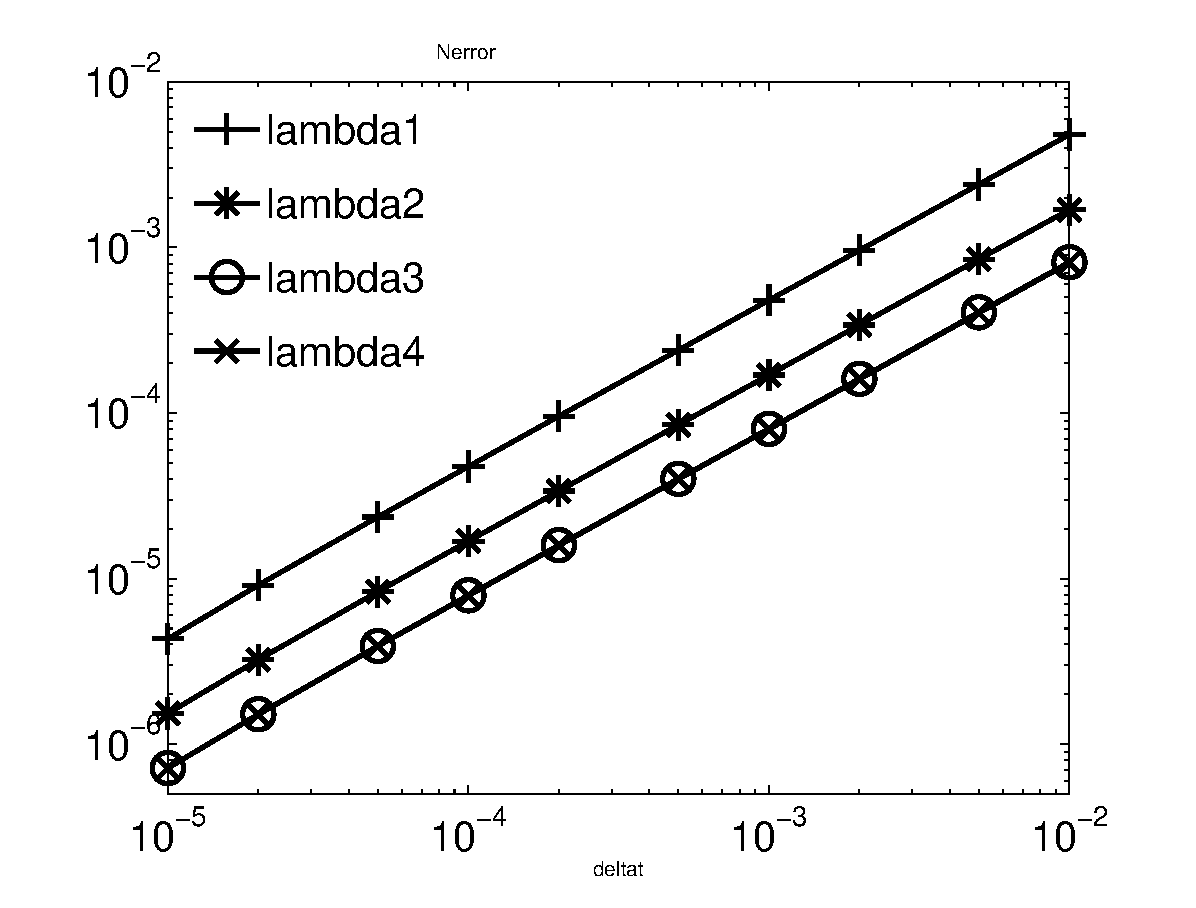
\includegraphics[scale=0.32]{lexample_fig3.eps}}
\subfigure{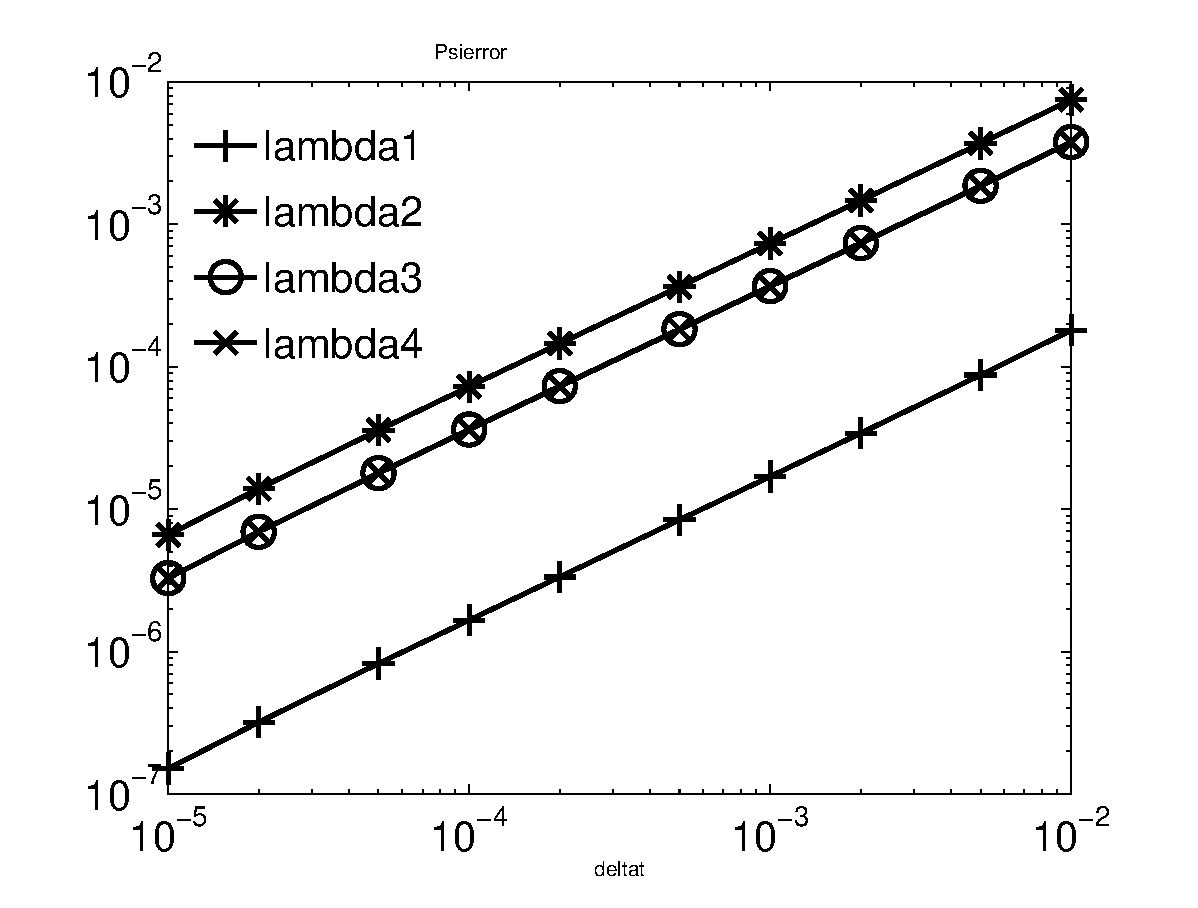
\includegraphics[scale=0.32]{lexample_fig4.eps}}
\caption{Note darker lines on this figure.}
\label{f2}
\end{figure}

In the second set of experiments, our purpose was to assess the 
relative amount of computational work required by the methods  
which use higher-order differencing to reach comparable levels  
of residual norm reduction. We compared pairs of methods EHA2  
and FD2, EHA4 and FD4, and EHA6 and FD6 by observing in each of 
20 trials the number of {\gmresm} iterations, number of $F$-evaluations,  
and run time required by each method to reduce the residual norm 
by a factor of $\e$, where for each pair of methods $\e$ was chosen  
to be somewhat greater than the limiting ratio of final to  
initial residual norms obtainable by the methods. In these trials,  
the initial approximate solutions were obtained by generating random  
components as in the similar experiments in section \ref{S2}. We note that for every  
method, the numbers of {\gmresm} iterations and $F$-evaluations required  
before termination did not vary at all over the 20 trials. The {\gmresm}
iteration counts, numbers of $F$-evaluations, and means and standard  
deviations of the run times are given in Table \ref{t1}. 
 
\begin{table}
\caption{Tables are to appear in $8$-point {\rm(}{\tt footnotesize}{\rm)} type.} 

\begin{center} {\footnotesize
\begin{tabular}{|c|c|c|c|c|c|} \hline  
&& Number of & Number of & Mean run time & Standard \\ 
Method & $\e$ & iterations & $F$-evaluations& (seconds) & deviation \\ \hline 
\lower.3ex\hbox{EHA2} & \lower.3ex\hbox{$10^{-10}$} & \lower.3ex\hbox{26} &  
\lower.3ex\hbox{32} & \lower.3ex\hbox{47.12} & \lower.3ex\hbox{.1048} \\ 
FD2 & $10^{-10}$ & 26 & 58 & 53.79 & .1829 \\ \hline  
\lower.3ex\hbox{EHA4} & \lower.3ex\hbox{$10^{-12}$} & \lower.3ex\hbox{30} &  
\lower.3ex\hbox{42} & \lower.3ex\hbox{56.76} & \lower.3ex\hbox{.1855} \\  
FD4 & $10^{-12}$ & 30 & 132 & 81.35 & .3730 \\ \hline  
\lower.3ex\hbox{EHA6} & \lower.3ex\hbox{$10^{-12}$} & \lower.3ex\hbox{30} &  
\lower.3ex\hbox{48} & \lower.3ex\hbox{58.56} & \lower.3ex\hbox{.1952} \\ 
FD6 & $10^{-12}$ & 30 & 198 & 100.6 & .3278 \\ \hline  
\end{tabular}}
\end{center} 
\label{t1} 
\end{table}  

In our first set of experiments, we took $c=d=10$ and used right 
preconditioning with a fast Poisson solver from {\fishpack}  
\cite{Swarztrauber-Sweet}, which is very effective for these  
fairly small values of $c$ and $d$. We first started each method 
with zero as the initial approximate solution and allowed it  
to run for 40 {\gmresm} iterations, after which the limit of residual  
norm reduction had been reached. Figure \ref{f2} shows plots  
of the logarithm of the Euclidean norm of the residual versus  
the number of {\gmresm} iterations for the three methods. We note
that in  Figure~\ref{f2} and in all other figures below, the plotted
residual norms were not the values maintained by {\gmresm}, but rather
were computed as accurately as possible ``from scratch.''  That is, 
at each {\gmresm} iteration, the current approximate solution was 
formed and its product with the coefficient matrix was subtracted 
from the right-hand side, all in double precision.  
It was important to compute the residual norms in this way because  
the values maintained by {\gmresm} become increasingly untrustworthy  
as the limits of residual norm reduction are neared; see \cite{Walker88}.  
It is seen in Figure~\ref{f2} that Algorithm EHA achieved  
the same ultimate level of residual norm reduction as the FDP  
method and required only a few more {\gmresm} iterations to do
so.  
 
In our second set of experiments, we took $c=d=100$ and carried out  
trials analogous to those in the first set above. No preconditioning  
was used in these experiments, both because we wanted to compare 
the methods without preconditioning and because the fast  
Poisson preconditioning used in the first set of experiments is 
not cost effective for these large values of $c$ and $d$. We first  
allowed each method to run for 600 {\gmresm} iterations, 
starting with zero as the initial approximate solution, after which  
the limit of residual norm reduction had been reached. 

\section{Numbering and linking within the article}
The SIAM macro numbers sections, environments, and equations by section.  Environments may be given single numbers 
by using the optional argument \texttt{onethmnum} in the \texttt{documentclass} command, and equations are single numbered
by including \texttt{oneeqnum}.  Tables and figures are given single numbers in the current SIAM macro to facilitate linking in the PDF.

\section{References}
References are usually numbered, but the author may also use a combination of letters and numbers in 
brackets after {\tt bibitem} to create reference identifiers of his or her choice.  Use of \texttt{natbib} is also permitted.

The aforementioned style manual contains many examples of preferred styles for different types of references.

\section{Supplemental material}
Authors should use the standard SIAM macro for supplemental material that resembles the normal article, such as appendices.  Ideally, numbered items should be prefaced
by the letter M (as in Theorem M.1).

\section*{Acknowledgments}
The authors thanks the anonymous authors whose work largely constitutes this example file. We are also thankful for the many
recommendations and suggestions that have made this macro example file what it is today.
 
 
\begin{thebibliography}{10} 
\bibitem{bs} {\sc R.~A. Brualdi and B.~L. Shader}, 
{\em On sign-nonsingular matrices and the conversion of the
permanent into the determinant}, in Applied Geometry and
Discrete Mathematics, The Victor Klee Festschrift, P.
Gritzmann and B. Sturmfels, eds., American Mathematical
Society, Providence, RI, 1991, pp. 117--134.
 
\bibitem{djd} {\sc J. Drew, C.~R. Johnson, and P. van den Driessche}, 
{\em Strong forms of nonsingularity}, Linear Algebra Appl.,
162 (1992), to appear. 
 
\bibitem{g} {\sc P.~M. Gibson}, {\em Conversion of the permanent into the 
determinant}, Proc. Amer. Math. Soc., 27 (1971),
pp.~471--476.
 
\bibitem{klm} 
{\sc V.~Klee, R.~Ladner, and R.~Manber}, {\it
Signsolvability revisited}, Linear Algebra Appl., 59
(1984), pp.~131--157.
 
\bibitem{m} 
{\sc K. Murota}, LU-{\em decomposition of a matrix with
entries of different kinds}, Linear Algebra Appl., 49
(1983), pp.~275--283.

\bibitem{Axelsson}
{\sc O.~Axelsson}, {\em Conjugate gradient type methods for unsymmetric and
  inconsistent systems of linear equations}, Linear Algebra Appl., 29 (1980),
  pp.~1--16.
  
\bibitem{BDM}
{\sc C. Bernardi, M. Dauge, and Y. Maday}, {\em Polynomials in the Sobolev
World}, \href{https://hal.archives-ouvertes.fr/hal-00153795v1}{https://hal.archives-ouvertes.fr/hal-00153795v1} (3 September 2007).

\bibitem{BMD09a}
{\sc C. Boutsidis, M.W. Mahoney, and P. Drineas},
 {\em An improved approximation algorithm for the column subset selection problem},
 in Proceedings of the 20th Annual ACM-SIAM Symposium on Discrete Algorithms (SODA), 2009, pp. 968--977.

\bibitem{Brown-Saad1}
{\sc P.~N. Brown and Y.~Saad}, {\em Hybrid {K}rylov methods for nonlinear
  systems of equations}, SIAM J. Sci. Statist. Comput., 11 (1990), 
  pp.~450--481.
  
\bibitem{Cswarm11}
{\sc I.~Chattopadhyay}, {\em Scalable $\epsilon$-optimal self-organization in
  communicating swarms using implicit probabilistic automata}, in \ Proceedings of the American
  Control Conference (ACC), IEEE Press, Piscataway, NJ, 2012, pp.~6047--6052.

\bibitem{DES}
{\sc R.~S. Dembo, S.~C. Eisenstat, and T.~Steihaug}, {\em Inexact {N}ewton
  methods}, SIAM J. Numer. Anal., 19 (1982), pp.~400--408.

\bibitem{EES}
{\sc S.~C. Eisenstat, H.~C. Elman, and M.~H. Schultz}, {\em Variational
  iterative methods for nonsymmetric systems of linear equations}, SIAM J.
  Numer. Anal., 20 (1983), pp.~345--357.

\bibitem{Elman}
{\sc H.~C. Elman}, {\em Iterative methods for large, sparse, nonsymmetric
  systems of linear equations}, Ph.D. thesis, Department of Computer
  Science, Yale University, New Haven, CT, 1982.

\bibitem{GloKR85}
{\sc R.~Glowinski, H.~B. Keller, and L.~Rheinhart}, {\em Continuation-conjugate
  gradient methods for the least-squares solution of nonlinear boundary value
  problems}, SIAM J. Sci. Statist. Comput., 6 (1985), pp.~793--832.

\bibitem{Golub-VanLoan}
{\sc G.~H. Golub and C.~F. Van~Loan}, {\em Matrix Computations}, 
  Second ed., The Johns  Hopkins University Press, Baltimore, MD,  1989.
  
\bibitem{LiZeng2012a}
{\sc C. P. Li and F. H. Zeng,}  {\em Finite difference methods for
fractional differential equations}, {Internat. J. Bifur.
Chaos Appl. Sci. Engrg.}, {22} (2012), 1230014.  

\bibitem{More}
{\sc J.~J. Mor\'e}, {\em A collection of nonlinear model problems}, in
  Computational Solutions of Nonlinear Systems of Equations, E.~L. Allgower and
  K.~Georg, eds., Lectures in Applied Mathematics, Vol. 26, American
  Mathematical Society, Providence, RI, 1990, pp.~723--762.

\bibitem{Saad}
{\sc Y.~Saad}, {\em Krylov subspace methods for solving large unsymmetric
  linear systems}, Math. Comp., 37 (1981), pp.~105--126.

\bibitem{Saad-Schultz}
{\sc Y.~Saad and M.~H. Schultz}, {\em {\rm GMRES}: A generalized minimal
  residual method for solving nonsymmetric linear systems}, SIAM J. Sci. Statist.
  Comput., 7 (1986), pp.~856--869.

\bibitem{SS13}
{\sc Cl.~Schillings and Ch.~Schwab}, {\em Sparsity in Bayesian inversion of parametric operator equations},
 Inverse Problems, 30 (2014), \href{http://dx.doi.org/10.1088/0266-5611/30/6/065007}{http://dx.doi.org/10.1088/0266-5611/30/6/065007}.

\bibitem{Swarztrauber-Sweet}
{\sc P.~N. Swarztrauber and R.~A. Sweet}, {\em Efficient {\rm FORTRAN}
  subprograms for the solution of elliptic partial differential equations}, ACM
  Trans. Math. Software, 5 (1979), pp.~352--364.

\bibitem{Walker88}
{\sc H.~F. Walker}, {\em Implementation of the {\rm GMRES} method using
  {H}ouseholder transformations}, SIAM J. Sci. Statist. Comput., 9 (1988),
  pp.~152--163.

\bibitem{Walker89}
{\sc H.~F. Walker}, {\em Implementations of
  the {\rm GMRES} method}, Computer Phys. Comm., 53 (1989),  pp.~311--320.

\end{thebibliography} 

\end{document} 

